\documentclass{article}
\usepackage[utf8]{inputenc}
\usepackage[spanish]{babel}
\usepackage{hyperref}
\usepackage{graphicx}
 
\hypersetup{
    colorlinks=true,
    linkcolor=blue,
    filecolor=magenta,      
    urlcolor=blue,
}

\usepackage{listings}
\usepackage{color}

\definecolor{codegreen}{rgb}{0,0.6,0}
\definecolor{codegray}{rgb}{0.5,0.5,0.5}
\definecolor{codepurple}{rgb}{0.58,0,0.82}
\definecolor{backcolour}{rgb}{0.95,0.95,0.92}
\lstdefinestyle{mystyle}{
    backgroundcolor=\color{backcolour}, commentstyle=\color{codegreen}, keywordstyle=\color{magenta},
    numberstyle=\tiny\color{codegray}, stringstyle=\color{codepurple}, basicstyle=\footnotesize,
    breakatwhitespace=false, breaklines=true, captionpos=b, keepspaces=true, numbers=left,                    
    numbersep=5pt, showspaces=false, showstringspaces=false, showtabs=false,tabsize=2
}
\lstset{style=mystyle}

\title{Tarea 12}
\author{fl.gomez10 at uniandes.edu.co}
%\date{March 2019}

\begin{document}

\maketitle

Horario de atención: Principalmente de 2:00pm a 5:00pm en la oficina i-109.
También se pueden enviar dudas al correo electrónico.
Entregar antes de finalizar la clase. 

Trabaje iniciando  sesión en la máquina virtual en línea
\href{https://mybinder.org/v2/gh/ComputoCienciasUniandes/FISI2026-201910/master?urlpath=lab}{mybinder.org/}
\footnote{\url{https://mybinder.org/v2/gh/ComputoCienciasUniandes/FISI2026-201910/master?urlpath=lab}}. 


\section{Ejercicio 1 (40 puntos) Trabajo en Casa - Integrar una función bidimensional con método Monte Carlo.}

Se tiene la función:
\begin{equation}
  f(x,y) = \sin \left(2 \pi x \right) e^{-(x^2 + y^2)/(\pi^2)} + 5
\end{equation}

\begin{itemize}
\item (10 pts) Use \texttt{scipy.integrate.dblquad} para integrar. Este será nuestro valor de referencia.
\item (30 pts) Evaluar la integral en $x \in(-5,5)$ e $y \in (-3,3)$ usando un método Monte Carlo de integración.
  Ajuste su método para tener un error absoluto inferior al $2\%$ respecto al valor de referencia.
\end{itemize}

Se tienen  $x_{min}$, $x_{max}$, $y_{min}$ e $y_{max}$. Se puede definir $z_{min}=0$, y se puede
calcular $z_{max}$ como el valor más grande que pueda tomar $f(x,y)$ dentro del domino, o puede
ser un valor ligeramente mayor.

Se puede definir alto, largo y ancho como las longitudes $L = w_{max} - w_{min}$ (con $w=\{x,y,z\}$).
El volumen del paralelepípedo se calcula como alto por largo por ancho.

Se genera una muestra de puntos aleatorios dentro del paralelepípedo.

Para cada punto aleatorio con coordenadas $(x,y,z)$ se evalúa si está debajo de la
superficie definida por $f(x,y)$, esto es, evaluar si  $z \leq f(x,y)$. Se lleva la
cuenta de cuántos puntos cumplen esta condición.

Al final, la integral de $f(x,y)$ será igual al volumen del paralelepípedo por la fracción
de puntos que están debajo de $f(x,y)$.


\section{Ejercicio 2 (60 puntos) - Muestreo con el algorigmo Metropolis-Hastings}

La variable x está definida dentro del dominio real $(-10,10)$.
Se tiene una distribución de probabilidad no normalizada $f(x)$ definida como:

\begin{equation}
  f(x) = 100 - x^2
\end{equation}

Implemente el método de Metropolis-Hastings para hacer un muestreo de $N=100000$ puntos.

Se genera un caminante aleatorio (Random Walk) que da cada paso según la función $f(x)$ y la posición
actual del caminante (Cadena de Markov). El decidir si se da el siguiente paso aleatorio
o si se permanece en la posición actual se realiza según el algoritmo de Metropolis y Hastings. 


\begin{itemize}
\item (5 pts) Implemente la función $f(x)$. (Pro-tip: Puede asignar \texttt{-np.inf} a valores
  de x fuera de dominio).
\item Inicie la lista de sampleo ``walk'' con un valor aleatorio $x_0$ dentro del dominio.
\item (5 pts) Defina un $\Delta x$ usando \texttt{random.rand()}, centrado en cero, con una amplitud
  que pueda variar. Este será el tamaño del paso que dará el caminante aleatorio, debe ser
  igual hacia la derecha o hacia la izquierda.
\end{itemize}

Una vez se han definido la función de probabilidad y se ha iniciado la lista de pasos del
caminante aleatorio, se define el ciclo principal de $N$ pasos. Preste especial atención a
los signos ($<$, $>$, $\geq$, $\leq$), de esto depende si funciona o no su Cadena de Markov
Monte Carlo (MCMC). (20 puntos)
\begin{itemize}
\item Defina $x_{old}$ como la última posición del caminante aleatorio
\item Genere $x_{new}$ como $x_{old}$ mas un $\Delta x$ (que puede ser positivo o negativo).
\item Evalúe $\alpha = f(x_{new}) / f(x_{old})$
\item Si $\alpha \geq 1$ entonces se guarda $x_{new}$ en la lista de posiciones del caminante y se repite el ciclo.
\item Si $\alpha<1$, se evalúa un número aleatorio $\beta \in [0,1)$, si $\beta \leq \alpha$ se acepta y se guarda
  $x_{new}$, con esto se da inicio a otro ciclo. En en caso contrario se rechaza $x_{new}$ y se guarda en la lista $x_{old}$.
\end{itemize}


Finalmente se realizan las gráficas. Vamos a revisar qué tan buena es la exploración que está realizando
nuestro caminante aleatorio.

\begin{itemize}
\item (10 pts) Defina un ancho muy pequeño $|\Delta x|  \sim 0.0001$ (el ancho del paso que da el caminante
  aleatorio). Graficar usando \texttt{plt.plot(walk)} y
  \texttt{plt.hist(walk, bins=np.linspace(-12,12,51))}
\item (10 pts) Reinicie ``walk'', defina ahora un ancho de paso muy grande $|\Delta x| \sim 100$.
  Graficar usando \texttt{plt.plot(walk)} y \\   \texttt{plt.hist(walk, bins=np.linspace(-12,12,51))}
\item (10 pts) Reinicie ``walk'', defina un ancho de paso apropiado para el dominio de la función que estamos
  estudiando. Graficar usando \texttt{plt.plot(walk)} y   \texttt{plt.hist(walk, bins=np.linspace(-12,12,51))}
\end{itemize}

Se espera obtener algo como esto:

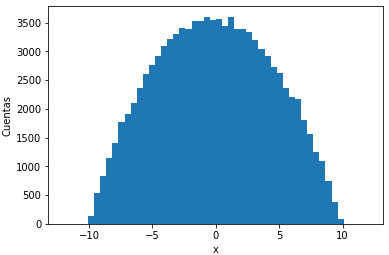
\includegraphics{hw12_hist.png}

Más información sobre cadenas de Markov y el diagnóstico de convergencia en esta presentación:
\url{http://halweb.uc3m.es/esp/Personal/personas/causin/esp/2012-2013/SMB/Tema8.pdf}

\end{document}
